\begin{frame}
	\only<1->{
	\begin{block}{Ecuacion de Burgers' Estocastica}
	\begin{equation*}
		d X(\xi, t) = \left[\alpha \partial_{\xi}^2 X(\xi, t) + \frac{1}{2} \partial_\xi \left(X^2 (\xi, t)\right) \right] dt + dW_t (\xi, t), \hspace{0.2cm} \xi \in [0, 1] 
	\end{equation*}
	con las condiciones de frontera e iniciales
	\begin{align*}
		X(0, t) &= X(1, t) = 0 , \hspace{2mm} t > 0, \\
		X(\xi, 0) &= x(\xi), \hspace{2mm}  x \in \mathcal{H},
	\end{align*}
	\end{block}
	}
	\only<2->{
	La ecuacion anterior se asocia a la ecuacion estocastica
	\begin{align*}
		dX &= [AX + B(X)]dt + dW_t \\
		X(0) &= x, \hspace{0.2cm} x \in \mathcal{H}
	\end{align*}
	}
\end{frame}	

\begin{frame}	
	\only<1->{
	Primeramente para obtener la solucion numerica, se define la funcion
	\begin{equation*}
		u(x, t) = \mathbb{E} \left[ u_0 (X^x_t) \right], 
	\end{equation*}
	}
	\only<2->{
	 
	\begin{block}{Ecuacion de Kolmogorov}
	\begin{equation*}
		\frac{\partial u}{\partial t} = \frac{1}{2} Tr(QD^2 u) + \langle Ax, Du\rangle_{\mathcal{H}} + \langle B(x), Du\rangle_{\mathcal{H}}, \hspace{0.1cm} x \in D(A)
	\end{equation*}
	\end{block}
	}
\end{frame}

\begin{frame}
	La solucion espectral esta dada como
	\begin{align*}
		u(t, x) = \displaystyle \sum _{n \in \mathcal{J}} u_{n}(t) H_n (x), \hspace{0.1cm} x \in \mathcal{H}, \hspace{0.1cm} t \in [0, T],
	\end{align*}		
	
	substituyendo en la ecuacion de Kolmogorov 
	\begin{equation*}
		\dot{u}_{m} (t) = -u_{m} (t) \lambda_{m} + \displaystyle \sum _{n \in \mathcal{J}} u_{n} (t) C_{n, m} , \hspace{0.1cm} n, m \in \mathcal{J}
	\end{equation*}
	\begin{equation*}
		\mathcal{J} = \{\alpha = (\alpha_i,i \geq 1) | \alpha_i \in \mathbb{N}\cup \{0\}, |\alpha|:= \displaystyle \sum _{i = 0}^{\infty}\alpha_i < \infty\}
	\end{equation*}
\end{frame}

\begin{frame}	
	Para las soluciones numericas definimos 
	\begin{equation*}
		J^{M, N} = \{\gamma = (\gamma_i, \hspace{1mm} 1 \leq i \leq M  ) \hspace{1mm} | \hspace{1mm} \gamma_i \in \{0, 1, \cdots, N \} \}
	\end{equation*}
	
	Entonces la solucion truncada es 
	\begin{equation*}
		\hat{u}_N (x, t) = \displaystyle \sum_{ n \in J^{M, N} } u_n (t) H_n (x), \hspace{2mm} x \in \mathcal{H}, \hspace{2mm}, t \in [0, T].
	\end{equation*}
	
	para obtener
	\begin{equation*}
		\dot{u}_{m} (t) = -u_{m} (t) \lambda_{m} + \displaystyle \sum _{n \in S_N} u_{n} (t) \bar{C}_{n, m} , \hspace{0.1cm} n, m \in S_N
	\end{equation*}
\end{frame}
	
\begin{frame}	
	Reescribiendo el sistema
	\begin{equation*}
		U^M (t) =
		\begin{pmatrix}
		u_{m_1} (t) & u_{m_2} (t) & \dots & u_{m_M} (t)
		\end{pmatrix}^T   
	\end{equation*}
	\begin{equation*}
		\dot{U}^M (t) =
		\begin{pmatrix}
		\dot{u}_{m_1} (t) & \dot{u}_{m_2} (t) & \dots & \dot{u}_{m_M} (t)
		\end{pmatrix}^T   
	\end{equation*}
	
	\begin{equation*}
		A =
		\begin{pmatrix}
		-\lambda_1 + C_{1,1} & C_{2,1} & \dots & C_{M-1,1} & C_{M,1} 
		\\
		C_{1,2} & -\lambda_2 + C_{2,2} & \dots & C_{M-1,2} & C_{M,2}  
		\\
		\vdots & \vdots & \ddots & \vdots & \vdots
		\\
		C_{1,M-1} & C_{2,M-1} & \dots & -\lambda_{M-1} + C_{M-1,M-1} & C_{M,M-1} 
		\\
		C_{1,M} & C_{2,M} & \dots & C_{M-1,M} & -\lambda_{M} + C_{M,M} 
		\end{pmatrix}
	\end{equation*}
\end{frame}
	
\begin{frame}
	Representacion matricial del sistema
	\begin{equation*}
		\dot{U}^M (t) = AU^M (t)
	\end{equation*}
	La cual tiene como solucion
	\begin{equation*}
		U^M (t) = \displaystyle \sum _{j = 1}^{M} c_i V_i e^{\eta_i t}
	\end{equation*}
	
	Eigenvectores y eigenvalores
	\begin{align*}
		V &= a + i b \\
		\eta &= \beta + i \mu
	\end{align*}
\end{frame}

\begin{frame}
	\begin{equation*}	
	\begin{pmatrix}
	u_1 (0) \\ u_2 (0) \\ \vdots \\ u_{M-1} (0) \\	u_M (0)
	\end{pmatrix}
	= 
	\begin{pmatrix}
	V1 & V2 & \dots & V_{M-1} & V_M
	\end{pmatrix}
	\begin{pmatrix}
	c_1 \\ c_2 \\ \vdots \\ c_{M-1} \\ c_M
	\end{pmatrix}
	\end{equation*}
	
	\begin{equation*}
	\begin{pmatrix}
	c_1 \\ c_2 \\ \vdots \\ c_{M-1} \\ c_M 
	\end{pmatrix}
	=	
	\begin{pmatrix}
	V1 & V2 & \dots & V_{M-1} & V_M
	\end{pmatrix}^{-1}
	\begin{pmatrix}
	u_1 (0) \\ u_2 (0) \\ \vdots \\ u_{M-1} (0) \\	u_M (0)
	\end{pmatrix}
	\end{equation*}
\end{frame}

\begin{frame}
	En los siguientes resultados se considero $x(\xi)$ como condicion inicial, y su expansion truncada de Chebyshev como una segunda condicion inicial
	\begin{align*}
		x(\xi) = \sin(\pi \xi), \hspace{3mm} y(\xi) = \displaystyle \sum^{N}_{k=0} c_k T_k (\xi),
	\end{align*}
	Usando una discretizacion espacial $\xi$ de $2048$ puntos en el intervalo $[0, 1]$, $1024$ puntos en la variable $t$ sobre el intervalo $[0, 10]$, considerando los parametros $\alpha = 0.01$, $N = 5$, $M = 11$.
\end{frame}

\begin{frame}	
	\centering	
	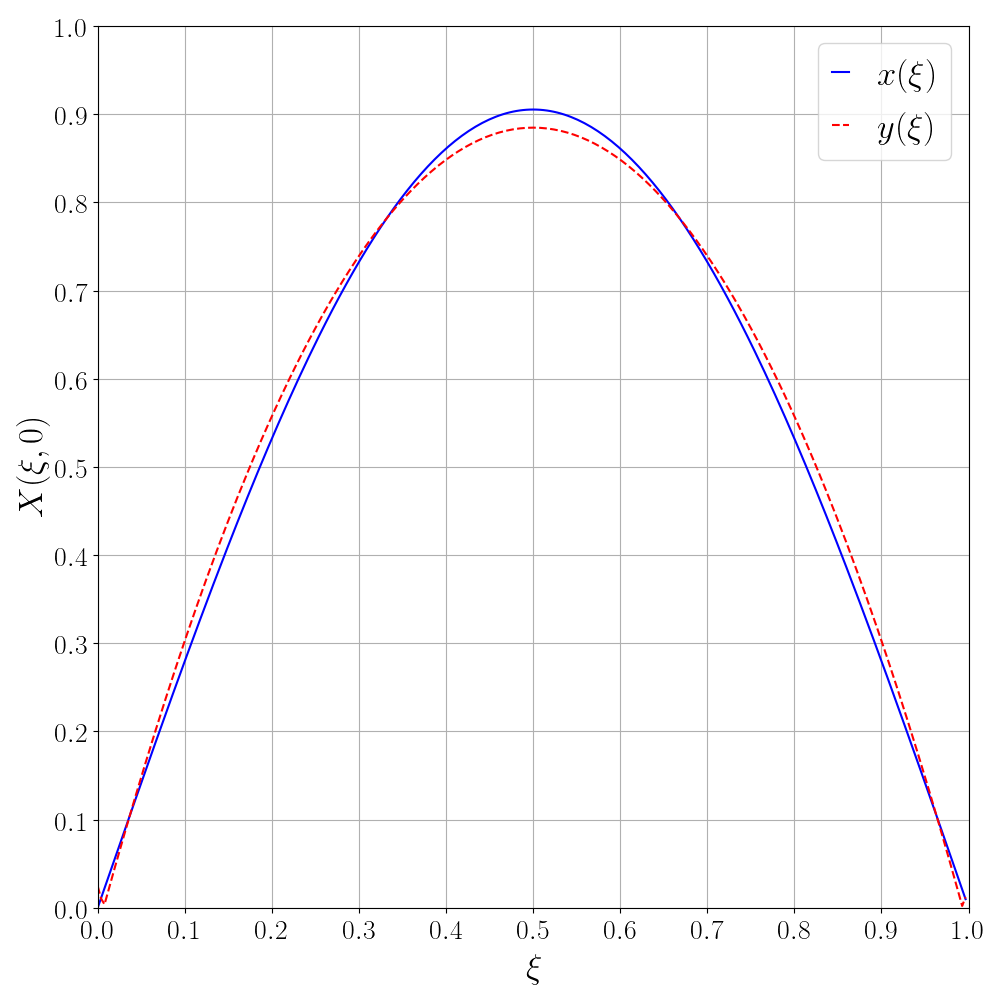
\includegraphics[width=8cm]{FIGURES/IC.png}
\end{frame}

\begin{frame}
	\centering
	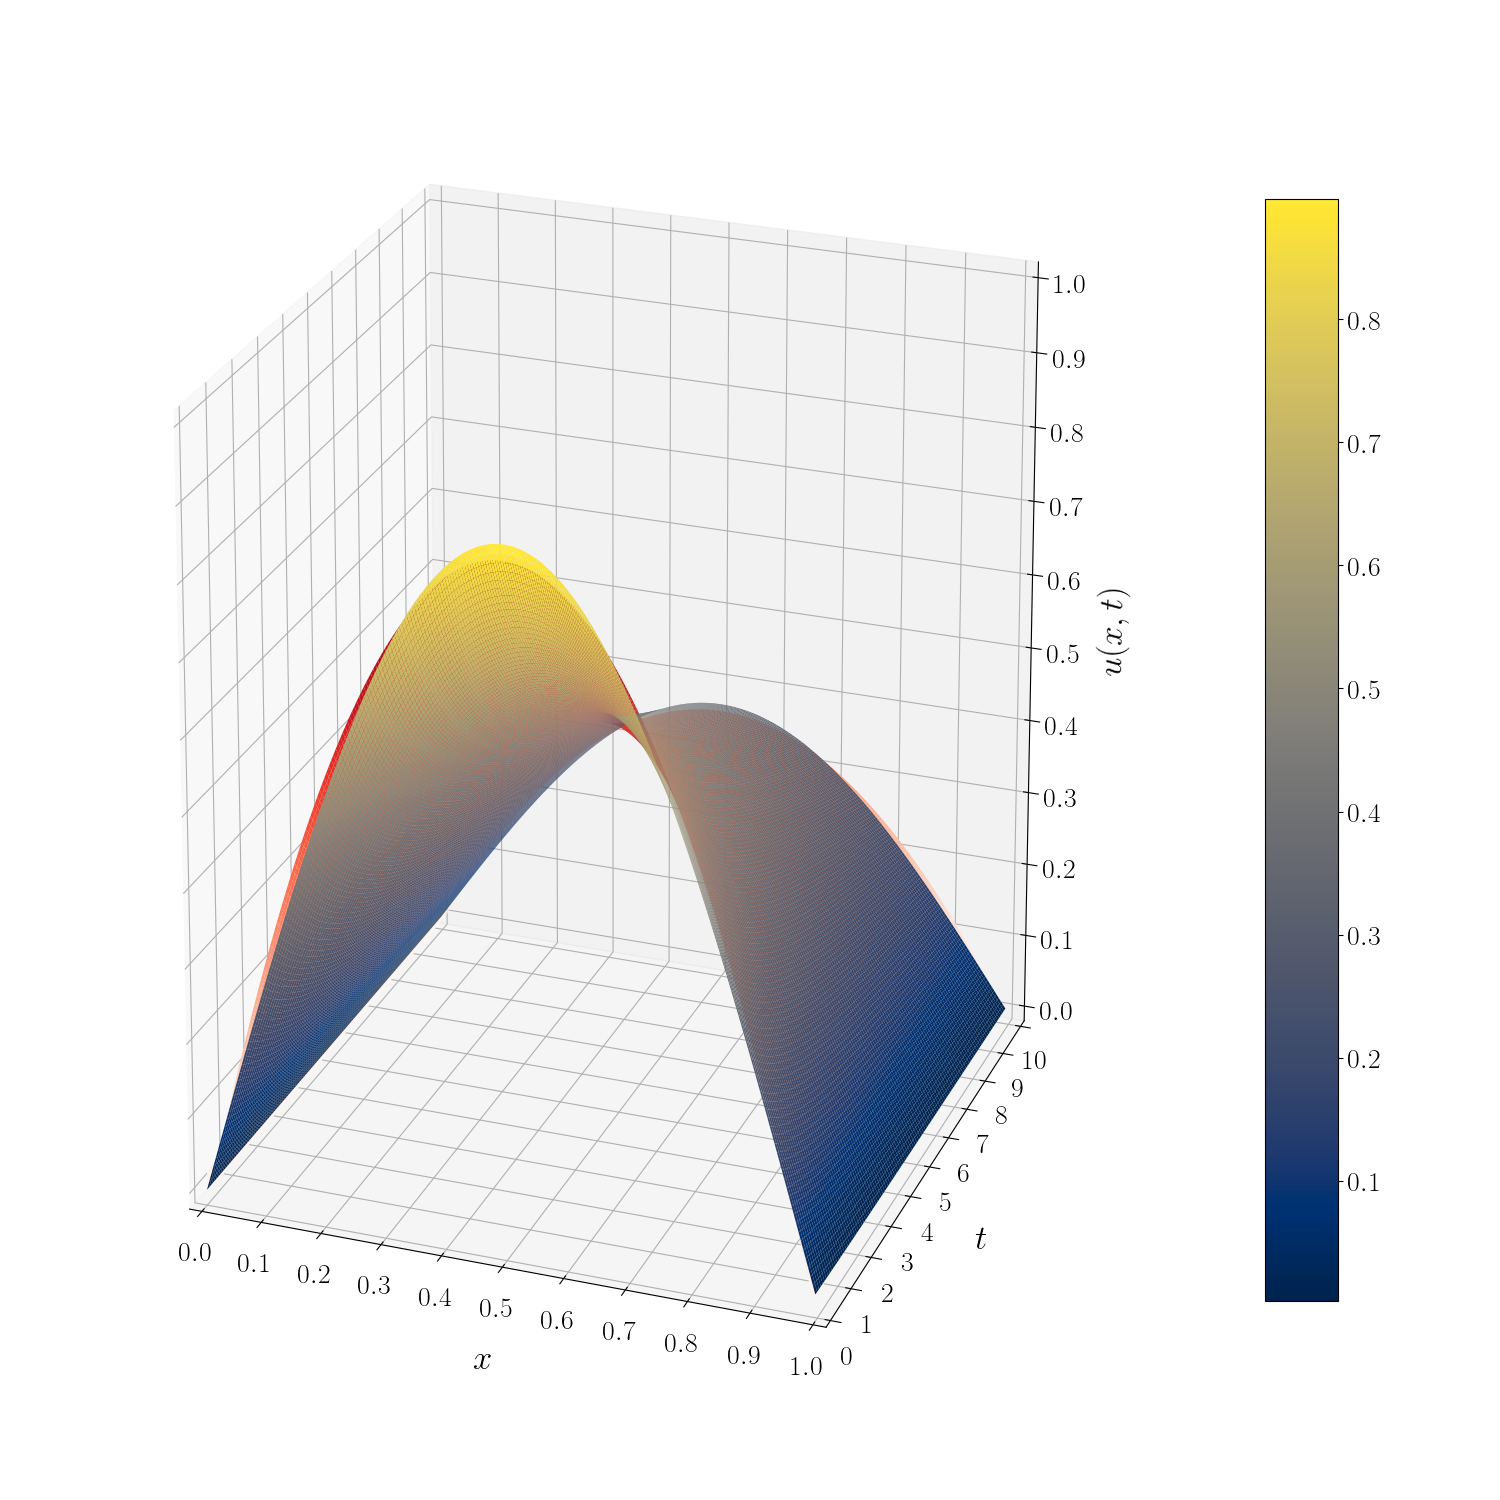
\includegraphics[width=8.5cm]{FIGURES/Numerical_Solution_Stochastic.png}
\end{frame}

\begin{frame}	
	\centering
	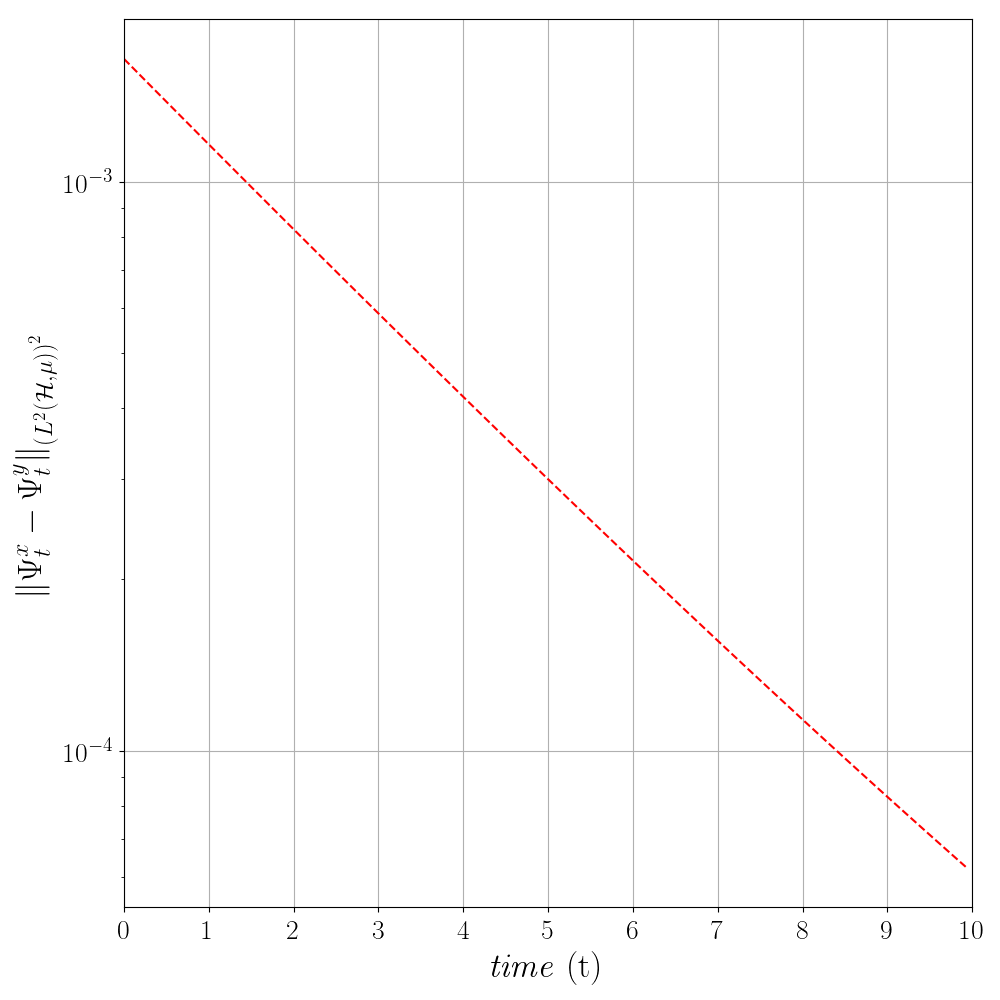
\includegraphics[width=7.5cm]{FIGURES/norms.png}
\end{frame}